\documentclass{article}
\usepackage{imakeidx}
\usepackage{graphicx}
\usepackage{wrapfig}
\usepackage{mathtools}
\graphicspath{{images/}}
\usepackage{geometry}
\geometry{a4paper,
total={170mm, 257mm},
left = 30mm,
right = 30mm,
bottom = 30mm,
top = 30mm
}

\usepackage{multicol}
\title{Computational Vision \linebreak Revision Notes}
\author{James Brown}
\makeindex
\begin{document}
	\pagenumbering{gobble}
	\maketitle
	\newpage
	\tableofcontents
	\newpage
	\pagenumbering{arabic}

	\section{Introduction}
	These are notes I have written in preparation of the 2017 Computation Vision exam. This year the module was run by Hamid Deghani (H.Dehghani@cs.bham.ac.uk).
	\linebreak \linebreak
	Computational vision is the acquisition of knowledge about objects and events in the environment through information processing of light emitted or reflected from objects. In short - we want to make a computer know what is where, by looking through information. We can also use computational vision to do automatic inference of properties of the world from images.

	\section{Human Vision}
	\par
	As humans we have evolved eyes which perceive the visible section of the electromagnetic spectrum, which falls between the wavelengths of 380nm - 760nm. Red light lies at the longer end (760nm) of visible light, and purple at the shorter end (380nm). \index{visible light}Visible light is strongly absorbed in the human eye because it can cause an electron to jump to a higher energy levels - yet it does not have enough energy to ionize cells. The evolutionary process of evolving eyes began more than 3 billion years ago with the formation of photopigments. These are molecules where light incident upon them will trigger a physical or chemical change. \index{photopigment}Photopigments capture photons which lead to the release of energy in the photopigment. This is may be used for photosynthesis or a behavioural reaction (a nerve reaction). A single \index{photocell}photocell contains multiple layers to catch light, not just one. This increases the chance of catching any one individual photon - if it's not caught by the first layer it's much more likely to be caught by the second and so on.

	\subsection{Image Formation}
	Photocells contain a light sensitive patch of photopigments. Using a single cell we can capture light in 1 dimension, but we can't really 'see'. All we can do is tell if the light is on, or off. With multiple cells we can have better direction resolution and with multiple cells we have a very wide aperture - we can't tell exactly where the image is. The image formed will be very bright but extremely fuzzy. This became curved over time and this which really helped with direction resolution as light incident on the left side of the curve must have come from the right. Images formed this way are still very blurry and will result in multiple projections of the same image. Over time eyes evolved to become \index{pinhole camera}pinhole cameras which form sharp yet dim images by allowing light to come from a single source (the pinhole) - effectively throwing away loads of potential information about the image. The solution to form sharp and bright images was to use a \index{lens}lens at the front of the eye. The lens focuses all incoming light to a single point and from there we can use our simple pinhole camera for forming images. It should be noted that the image formed is upside down to what exists in reality.
	
	\subsection{Retina Processing}
	The human \index{retina}retina contains two kinds of \index{photoreceptors}photoreceptors which respond to incident light - \index{rods}\textbf{rods}  (around 120 million) and \index{cones}\textbf{cones} (around 6 million). Rods are extremely sensitive photosensors and respond to a single photon of light. Multiple rod cells converge to the same \index{ganglion cell}ganglion cell and therefore neuron within the \index{retina} which results in poor spatial resolution. Rods are responsible simply for detecting the presence of light, and as a result make up the entirety of our night-vision. On the other hand, cones are active at much higher light levels and responsible for the detection of different colours of light. Cones have a much higher resolution as they are processed by several different neurons. Within the eye we have a \index{receptive field}receptive field, which is the area on which light must fall for a neuron to be stimulated. It should be noted that receptive field in the center of the eye is much smaller than it is for the periphery of the eye.
	
	\par There are two kinds of \textbf{ganglion cell}\index{ganglion cell} - on-center and off-center. On-center ganglion cells are stimulated when the center of its receptive field is exposed to light and is inhibited when the surround is exposed to light. Off-center ganglion cells have the exact opposite response to on-center ganglion cells. The difference between on-center and off-center ganglion cells allows them to transmit information not just about whether the photorecptor cells are firing but also about the firing rates of the center and surround of the receptive field - they can transmit information about contrast.
	
	\begin{figure}[ht]
		\centering
		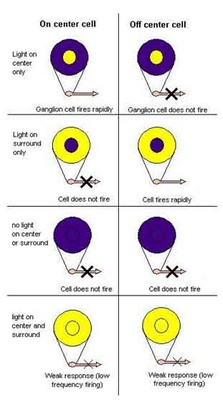
\includegraphics[width=0.4\textwidth]{on_off_ganglion_cells}
		\caption{How on-center and off-center ganglion cells respond to light}
		\label{fig:on off ganglion}
	\end{figure}
	
	\subsection{The Visual Pathway}
	Vision is generated by photoreceptors in the retina. All the information captured leaves the eye by way of the optic nerve\index{optic nerve}. There is a partial crossing of axons at the optic chiasm\index{chiasm}. This is only partial as information from both eyes is sent to both sides of the brain - this allows us to process depth. After this chiasm, the axons are called the optic tract. The optic tract wraps around the midbrain to get to the lateral geniculate nucleus (LGN)\index{lateral geniculate nucleus}. The LGN axons fan out through the deep white matter of the brain and ultimately to the visual cortex\index{visual cortex}.
	\begin{figure}[h]
		\centering
		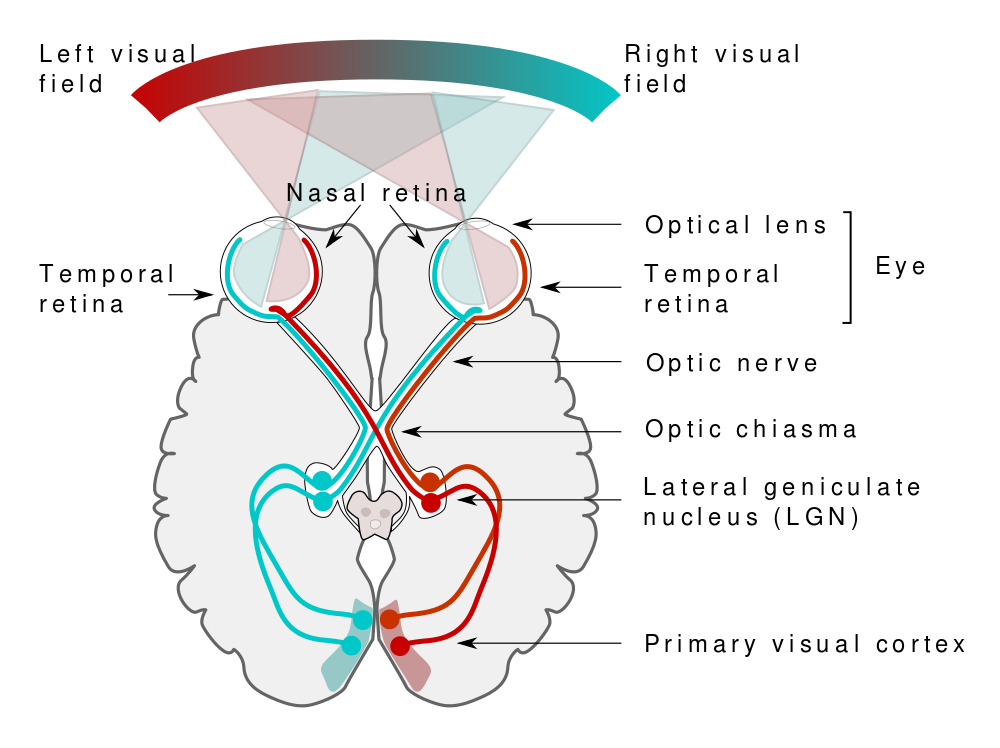
\includegraphics[width=0.6\textwidth]{visual_pathway}
		\caption{The visual pathway in the human brain}
		\label{fig:visual pathway}
	\end{figure}
	
	\subsection{Colour Processing}
	Objects in the world selectively absorb some wavelengths (a colour) and reflect other wavelengths. Human retinas contain three different types of cones to respond to different colours. This gives us the ability to distinguish different forms of the same object - for example: unripe, ripe and off fruit. Many theories of colour vision have been proposed and some have been hard to disprove until recently. 
	\par	
	In 1802 Young proposed that the eye has three different types of receptors, each of which are sensitive to a single hue. From this he proposed that any colour can be produced by appropriate mixing of the three primary colours. This is known as the trichromatic theory\index{trichromatic theory}.
	
	\par 
	Hering suggested that colour may be represented in a visual system as 'opponent colours' in the 1930's.
	
	
	\section{Edge Detection}
	\subsection{Intensity Images}
	An intensity image\index{intensity image} is a data matrix whose values represent intensities within some range. Each element of the matrix corresponds to one image pixel\index{pixel}. An indexed image consists of a data matrix, $X$, and a colour map\index{colour map} matrix, $map$. $map$ is a $m$-by-3 array of double containing floating point values in the range $[0, 1]$. Each row in the map specifies the red, green an blue components of a single color. Each cell in the indexed image then specifies the corresponding colour from the colour map. An intensity image can be thought of as a function $f(x, y)$ mapping coordinates to intensity. From this we can calculate an intensity gradient\index{intensity gradient}.
	\begingroup
	\renewcommand*{\arraystretch}{1.5}
	\[ \overrightarrow{G}[f(x,y)] = \begin{bmatrix}G_{x} \\ G_{y} \end{bmatrix} = \begin{bmatrix} \frac{df}{dx} \\ \frac{df}{dy} \end{bmatrix} \]	
	\endgroup

	 This is a vector which we can think of as having an $x$ and $y$ component. We can calculate both the magnitude and direction for this gradient of intensity. 
	\begin{multicols}{2}
		\noindent
		\centering
			$M(\overrightarrow{G}) = \sqrt{G_{x}^{2} + G_{y}^{2}}$ \\
			$\alpha(x, y) = \tan^{-1}\left(\frac{G_y}{G_x}\right)$
	\end{multicols}
	
	When calculating the magnitude, figuring out a square root can be very computationally expensive. It's possible to replace this with an approximation: $M(\overrightarrow{G}) = |G_{x}| + |G_{y}|$
	
	\subsection{Approximating the Intensity Gradient}
	In order to approximate the gradient we may use a variety of different masks over the image, such as the Roberts and Sobel detectors. These masks use the idea of convolution in order to calculate the rate of change of intensity at each pixel. 
	
	\begin{figure}[ht]
		\begin{minipage}[b]{.23\textwidth}
			\begingroup
			\renewcommand*{\arraystretch}{1.7}	
			\centering
			\[ \begin{bmatrix} -1 & 0 & 1 \\
								-2 & 0 & 2 \\
								-1 & 0 & 1
			\end{bmatrix} \]
			\endgroup
			\caption{Sobel X mask}
			\label{fig:sobel x mask}
		\end{minipage}
		\hfill
		\begin{minipage}[b]{.23\textwidth}
			\begingroup
			\renewcommand*{\arraystretch}{1.7}	
			\centering
			\[ \begin{bmatrix} 1 & 2 & 1 \\
								0 & 0 & 0 \\
								-1 & -2 & -1
			\end{bmatrix} \]
			\endgroup
			\caption{Sobel Y mask}
			\label{fig:sobel y mask}
		\end{minipage}
		\hfill
		\begin{minipage}[b]{.23\textwidth}
			\begingroup
			\renewcommand*{\arraystretch}{1.7}	
			\centering
			\[ \begin{bmatrix} 1 & 0 \\
								0 & -1
			\end{bmatrix} \]
			\endgroup
			\caption{Roberts X mask}
			\label{fig:roberts x mask}
		\end{minipage}
		\hfill
		\begin{minipage}[b]{.23\textwidth}
			\begingroup
			\renewcommand*{\arraystretch}{1.7}	
			\centering
			\[ \begin{bmatrix} 0 & -1 \\
								1 & 0
			\end{bmatrix} \]
			\endgroup
			\caption{Roberts Y mask}
			\label{fig:roberts y mask}
		\end{minipage}
		
	\end{figure}
	
	Convolution is the computation of weighted sums of image pixels. For each pixel in the image, the new value is calculated by translating the mask to the pixel and taking the weighted sum of all the pixels in the neighbourhood. Once we have a value for the rate of change of the intensity gradient we can threshold our image to produce the locations of edges.
	
	\section{Noise Filtering}
	When taking images we also gather a lot of noise which results in fake edges once we apply our edge detectors. We would like to remove this noise and we have many filters which can be implemented by the idea of convolution. The most widely used of these filters is the Gaussian filter\index{gaussian filter}, although there are other simpler filters such as the mean filter\index{mean filter}.
	\begin{figure}[ht]
	\begin{minipage}{.5\textwidth}
			\begingroup
			\renewcommand*{\arraystretch}{1.7}	
			\centering
			\[ \begin{bmatrix} \frac{1}{9} & \frac{1}{9} & \frac{1}{9} \\
								\frac{1}{9} & \frac{1}{9} & \frac{1}{9} \\
								\frac{1}{9} & \frac{1}{9} & \frac{1}{9}
			\end{bmatrix} \]
			\endgroup
			\caption{An example mean filter}
			\label{fig:mean filter}
	\end{minipage}
	\begin{minipage}{.5\textwidth}
		\centering
		\[ \begin{bmatrix} 0 & .01 & .02 & .01 & 0 \\
								.01 & .06 & .11 & .06 & .01 \\ 
							    .02 & .11 & .16 & .11 & .02 \\
							    .01 & .06 & .11 & .06 & .01 \\
							    0 & .01 & .02 & .01 & 0
				\end{bmatrix} \]
		\caption{An example Gaussian filter}
		\label{fig:gaussian filter}

	\end{minipage}
	\end{figure}
	
	The mean filter averages a pixels value with all of the surrounding intensities for a new value. A Gaussian filter follows the same principle as this but uses a weighting, valuing pixels closer to the original more than pixels farther away.	The Gaussian filter has an extra bonus of being able to be applied as two individual 1D Gaussian filters in sequence rather than one large 2D filter as shown below. Applying two smaller 1D filters in sequence is much more efficient than a single, large 2D filter.
	\begin{figure}[ht]
	\begin{multicols}{2}
		\[\begin{bmatrix} 0.0545 & 0.2442 & 0.4026 & 0.2442 & 0.0545 \end{bmatrix} \] \\
		\[\begin{bmatrix} 0.0545 \\ 0.2442 \\ 0.4026 \\ 0.2442 \\ 0.0545 \end{bmatrix} \]
	\end{multicols}
	\caption{A Gaussian filter deconstructed to two 1D filters which can be applied in sequence}
	\label{fig:1d gaussian filter}
	\end{figure}
	
	\section{Advanced Edge Detection}
	Intensity changes can be caused by geometric events such as surface orientation discontinuities, depth discontinuities, color discontinuities and texture discontinuities. It can also be caused by non-geometric events such as illumination changes, specularities, shadows and inter-reflections. All of these events can be used to try to find edges in the image. When we try to detect edges, we are trying to produce a line 'drawing' of a scene from an image of that scene. We use this to extract important features of an image, such as corners and curves. These features are then used by higher-level computer vision algorithms.
	
	\subsection{Main steps in Edge Detection}
	Regardless of methods, there a few major steps to edge detection:
		\begin{enumerate}
			\item \textbf{Smoothing}: suppress as much noise as possible, without destroying any of the true edges.
			\item \textbf{Enhancement}: apply differentiation to enhance the quality of edges (i.e. sharpening).
			\item \textbf{Thresholding}: determine which edge pixels should be discarded as  noise and which should be retained (i.e. threshold edge magnitude).
			
			\item \textbf{Localization}: determine the exact edge location.
		\end{enumerate}

	\par
	Most of the time, points that lie on an edge are detected by 
		\begin{enumerate}
			\item Detecting the local \textit{maxima} or \textit{minima} of the first derivative.
			\item Detecting the \textit{zero-crossings}\index{zero crossing} of the second derivative
		\end{enumerate}
		
	There are a few practical issues that come with this. When smoothing an image, the smoothing effect achieved depends on the mask size (for example, with a Gaussian filter it depends on $\sigma$). A larger mask will reduce noise more, but it also worsens localization and adds uncertainty to the location of the edge.
	
	Based on this we can draw up some criteria for an optimal method of edge detection:
	\begin{enumerate}
		\item \textbf{Good detection}: Minimize the probability of false positives and false negatives (spurious edges and missing real edges).
		\item \textbf{Good localization}\index{localization}: Detected edges must be as close as possible to the true edges.
		\item \textbf{Single response}\index{single response}: Minimise the number of local maxima around the true edge.
	\end{enumerate}

	Canny showed that the first derivative of Gaussian closely approximates the operator that optimizes the product of signal-to-noise ratio\index{signal-to-noise ratio} and localization\index{localization}.

	\subsection{Hysteresis}
	Hysteresis thresholding\index{hysteresis thresholding} uses two thresholds - a low threshold $t_{l}$ and a high threshold $t_{h}$ (usually this is $2t_{l}$). This makes the assumption that important edges should be along continuous curves in the image. It allows us to follow a faint section of a given line and to discard a few noisy pixels that do not constitute a line but have produced large gradients. We begin by applying the high threshold - this marks edges that we can be fairly sure that are genuine. Starting from these points, and using the directional information derived earlier, edges can be traced throughout the whole image. While tracing an edge, we apply the lower threshold, allowing us to trace faint sections of edges as long as we find a starting point. 

	\section{Hough Transform}
	So far we haven't actually found edge segments, just lots and lots of edge points. The Hough Transform\index{hough transform} is a common approach to finding parametrised line segments. Every straight line in an image can be described by an equation. Each edge point in an image, if considered in isolation, could lie on an infinite number of straight lines. In Hough Transform each edge point votes for every line it could be on, and the lines with the most votes win.
	
	\par
	Any line can be represented by using just two numbers - $w$ and $\phi$ - as long as we have a fixed origin point that we describe all lines in relation to. We use $w$ as the distance away from the agreed origin and $\phi$ as the angle to the horizontal. Using these two values we can find a single point in space - we define the line we want to represent as passing through this point and perpendicular to our line which we used to define the point. 
	
	\par 
	Since we can define any line in the image space using $(w, \phi)$, we can represent any line in the image space as a point in the plane defined by $(w, \phi)$. The plane defined by $(w, \phi)$ is known as the \textbf{Hough space}\index{hough space}. We do this for all possible (or as many as we feasibly can do) lines that could pass through the point in the image space, mapping them all to the Hough space. The result of this is a sinusoidal curve in the Hough space. When we expand this to mapping two points in the image space to the Hough space, we will have two sinusoidal curves in the Hough space. The intersection of these two curves has two 'votes' and represents the straight line in the image space that passes through both points. 	
	
	The Hough transform also has generalised versions versions for other geometric shapes, such as ellipses and circles.
	
	\par 
	We can sketch an algorithm to describe how the Hough transform works:
	
	\begin{verbatim}
	for each point (x, y)
	    for each angle p
	        w = x * cos(p) + y * sin(p)
	        A[p, w] = A[p, w] + 1
	    end
	end
	
	where A > Threshold return a line
	\end{verbatim}
	
	When using the straight line transform we need to suppress non-local maxima. We also need to make sure to apply edge thinning to our image before we apply the Hough transform.
	
	\section{Scale Invariant Feature Transform}
	We can now detect features in images. The most basic feature is edges, but through the use of Hough transform\index{hough transform} we can also detect lines and even geometric shapes such as circles. We want to detect features for various reasons, such as object recognition\index{object recognition}, wide baseline matching\index{wide baseline matching} and tracking\index{tracking}. In order to do this we need to make sure our features are invariant. Good features should be robust to all sorts of nastiness that can occur between two different images. There are many different causes of invariance:
	\begin{itemize}
		\item Illumination
		\item Scale
		\item Rotation
		\item Affine transformation (scaling and stretching)
		\item Full perspective
	\end{itemize}
	
	\subsection{Dealing with Illumination Invariance}
	The easiest way to achieve illumination invariance\index{illumination invariance} is to normalise the image. This is done by creating a histogram of all intensity values within the image. We can then stretch the histogram to match others of the same image in different illuminations (other images with different illumination should still have the same shape of histogram, even in not the exact same histogram). This stretch can be achieved through simple linear normalization.
	
	\subsection{Dealing with Scale Invariance}
	 One way to ensure our image is scale invariant\index{scale invariant} is by trying to scale it up and down, and see if a feature exists regardless of how much the image is scaled. There are two main methods to achieve this: Pyramids\index{pyramids} and Scale Space\index{scale space} (DOG method\index{DOG method}). 
	
	\par	 
	 In the pyramids method\index{pyramid method}, we divide the width and height of the image by 2. We take the average of 4 pixels for each new pixel and repeat this process until the image is very small. We can then run our filters (edge detectors) over the image to check for the existence of certain features. If the feature still exists all the way down, we can say that the feature is scale invariant. On the other hand, the DOG (Difference of Gaussian\index{difference of gaussian}) method is very similar to pyramids. Instead will fill the gaps with blurred images. This is like having a nice linear scaling without any expense. We take the features from the differences of the images, and if the feature is repeatably present in between Difference of Gaussians it is scale invariant and we should keep it.
	
	\subsection{Dealing with Rotational Invariance}
		We can deal with rotational invariance\index{rotational invariance} in much the same way as we deal with illumination invariance. We want to rotate all features to go in the same way in a determined manner. To do this, we take a histogram of all edge directions in the image and then rotate the image to the most dominant rotation (or possibly even the second most dominant if it's good enough).
		
	\section{Face Recognition}
	This section is about face recognition, not detection - we will not be taking an image and finding the face within.
	
	\subsection{Eigenfaces}
	We can have a face, which is a weighted combination of some parts or basis faces. The basis faces are called eigenfaces\index{eigenface}. The basis faces can be differently weighted to represent any face, so we can use different vectors of weights to represent different faces.
	
	\begin{figure}[h]
		\centering
		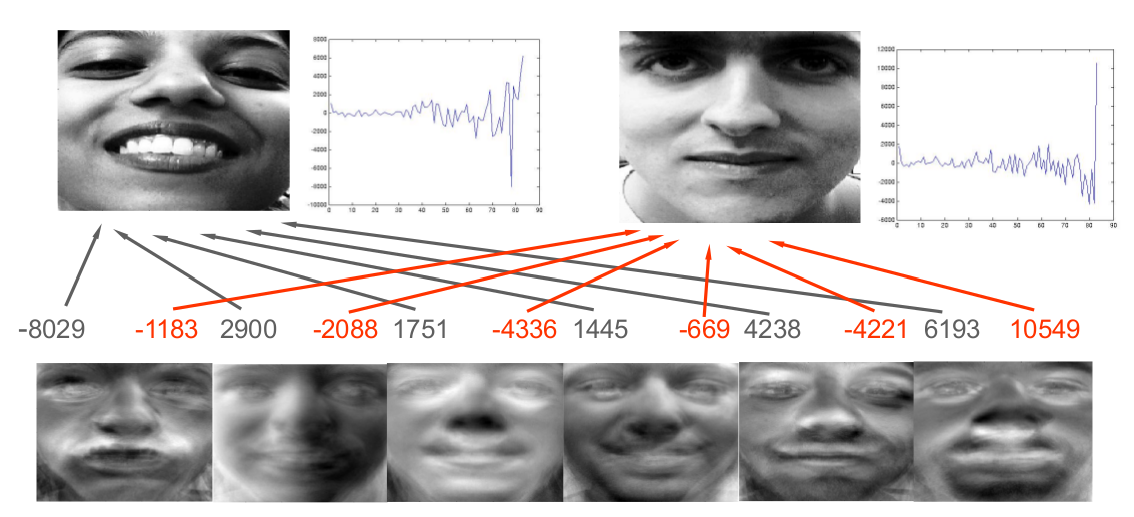
\includegraphics[width=\textwidth]{eigenfaces}
		\caption{A figure showing how to build any face from a set of basis faces}
		\label{fig:eigenfaces}
	\end{figure}
	
	Obviously we must pick the set of basis faces, and to do this we need a set of real training faces. From these we can then learn a set of basis faces which best represent the differences between each of the training faces. We'll use a statistical criterion for measuring the notion of 'best representation of the differences between training faces'. Then we can store each face as a set of weights from those basis faces.
	
	\subsection{Finding Eigenfaces}
	There are two possible ways we can use eigenfaces - firstly we can store and then reconstruct a face from a set of weights. Secondly we can recognise a new picture of a familiar face.
	
	Initially, we have to figure out how to learn eigenfaces. A method called principle components analysis (PCA) is used\index{principle components analysis}. In order to use this we have to understand what an eigenvector\index{eigenvector} is and also what covariance\index{covariance} is.
	
	To begin, we imagine that our face is simply a (high dimensional) vector of pixels. For humans it's easier to think about 2 dimensions, so we'll do just that and have our data in just two dimensions. When we have data in two dimensions, we only really need one dimension to represent it. To do this we can take a line through space, and then take the projection of each point onto that line - doing this means we have represented our data in 'one' dimension. The choice of line is important, some lines represent the data in this way well, and some badly. The projection onto some lines separates the data well, and the projection onto some lines separates it badly. However, rather than using a line we can perform roughly the same trick using a vector $v$. When using a vector, we instead have to scale the vector to obtain any point on the line and this vector is called an \textbf{eigenvector}\index{eigenvector}. The value $\mu$, which we use to project any point on the vector, is our \textbf{eigenvalue}\index{eigenvalue}.
	
		$\text{An eigenvector is a vector } v \text{ that obeys the rule } \mathbf{A}v = \mu v$ where $\mathbf{A}$ is a matrix, $\mu$ is a eigenvalue. A few rules about eigenvectors:
		\begin{itemize}
			\item We think of matrices as performing transformations on vectors
			\item We think of eigenvectors of a matrix as being special vectors that are scaled by that matrix
			\item Different matrices have different eigenvectors
			\item Only square matrices can have eigenvectors, and not all square matrices even have them
			\item An $n$ by $n$ matrix has at most $n$ different eigenvectors
			\item All the distinct eigenvectors of a matrix are orthogonal (perpendicular).
		\end{itemize}
		
	With our data, we need to find the vector which can be used to separate the points in our data as much as possible. This vector turns out to be the vector which expresses the direction of the correlation. The covariances then can be expressed as a matrix. The covariance of two variables is
	\[ cov(x_{1}, x_{2}) = \frac{\sum_{i=1}^{n}(x_{1}^{i} - \bar{x_{1}})(x_{2}^{i} - \bar{x_{2}})}{n - 1} \]	
	
	This covariance matrix has eigenvectors and eigenvalues. The largest eigenvalue shows you the most dominant vector (corresponding to the direction in which the data varies more). This is principle components analysis.
	
	\subsection{Using Eigenfaces}
	All we are going to do is treat the face as a point in a high dimensional space, and then treat the training set of face pictures as our set of points. In order to train, we calculate the covariance matrix of the faces and then find the eigenvectors of that covariance matrix. The found eigenvectors are the eigenfaces or basis faces. Eigenfaces with bigger values will explain more of the variation in the set of faces (they are more distinguishing).
	
	\par
	When we see an image of a face we can transform it to the face space with $\mathbf{W}_{k} = \mathbf{X}^{\mathbf{i}} . \mathit{v}_{k}$. There are $k=1...n$ eigenfaces $v_{k}$, and the $i^{\text{th}}$ face in the image space is a vector $x^{i}$ with corresponding weight $w_{k}$. We calculate the corresponding weight for every eigenface. Recognition is now simple, we can find the euclidean distance $d$ between our face and all the other stored faces in the face space with \[ d(w^{1}, w^{2}) = \sqrt{\sum_{i=1}^{n}(w_{i}^{1} - w_{i}^{2})^{2}} \]
	
	The closest face in the face space is the chosen match.
	\section{Motion}
	We aim to detect which changes have occurred in two different frames, and we can use this to deduce what motions have induced those changes. There are four possible possibilities for a dynamic camera and world:
	\begin{itemize}
		\item Stationary camera, stationary object
		\item Stationary camera, moving objects
		\item Moving camera, stationary object
		\item Moving camera, moving objects
	\end{itemize}
	
	But how do we detect changes? Firstly, we detect features in two different frames. Then simply look at the difference between features at time $t$ and time $t + 1$. Any differences in the two features, indicates that motion has occurred. More formally, we can say $F(x, y, i)$ is the intensity of the image at time $i$, at point $x, y$. It follows that the difference picture, $DP$, is defined as:
	\[ DP_{12}(x, y) = \begin{cases}
		1 \text{ if } |F(x, y, 1) - F(x, y, 2)| > \tau \\
		0 \text{ otherwise}
		\end{cases} \]
		
	This approach is not without issues. If we have random noise in the image, the difference image will include all the noise\index{noise} points in both images even if no motion\index{motion} has occurred at all. To solve this, we may want to filter out all pixels that are not part of some larger structure. We use the idea of connectedness\index{connectedness} to achieve this, in particular 4 or 8 connectedness. Two pixels can be said to be 4-neighbours\index{4-neighbours} is they share a common boundary. Two pixels are said to be 8-neighbours\index{8-neighbours} if they share at least one common corner. Two pixels are also 8-neighbours if we can create a path of 8-neighbours from one to the other. To remove noise, pixels that are not in a connected cluster of a certain size are removed from the difference image.
	
	\par 
	When determining motion, there is not enough information in the local intensity changes to give us the information that we want. This can be demonstrated via the aperture problem. When we only have a small area in which to observe, we cannot tell exactly what direction the object is moving (for example, something appearing to move down and right may only be moving to the right). This explains why edges are very bad for determining motion. To get around this we have to pick the particularly interesting areas of the image. Corners are a good example of particularly interesting areas. Once we have found these particularly interesting areas, we would like to match them between different images over time.
	
	\par 
	The Moravec operator\index{moravec operator} is a corner detector. It defines interest points as points where there is a large intensity variation in every direction, which is the case at corners. One side-effect is that it is very sensitive to detecting isolated pixels as corners.
	
	\par 
	Once we have points of interest, we try to match the points in one image with the points in another. Using this we can estimate the motion that has occurred. Motion correspondence\index{motion correspondence} is guided by three principles:
	\begin{enumerate}
		\item \textbf{Discreteness}\index{discreteness}: a measure of the distinctiveness of individual points
		\item \textbf{Similarity}\index{similarity}: a measure of how closely two points resemble one another
		\item \textbf{Consistency}\index{consistency}: a measure of how well a match conforms with nearby matches
	\end{enumerate}
	
	To calculate the degree of similarity between two patches take the sum of the squared differences in the pixel values (L1-norm - absolute difference).
	
	\[ w_{ij} = \frac{1}{1 + \alpha s_{ij}} \]
	
	When we want to try to match two patches, we calculate the weights for all the possible matches for patch i(t). How to calculate the weight is shown in the above equation. We assume some value for $\alpha$, such as $1$. Once we have all the weights, we normalise to produce probabilities for each of the patches to calculate the best matches between patches.
	

	\section{ROC Analysis}
	Receiver operating characteristic analysis provides us tools to select possibly optimal models and to discard suboptimal ones. In order to carry out ROC analysis we need to count the different kind of errors that are possible. When classifying if a pixel is an edge or not, there are 4 possible situations - \textbf{true positive} (predicted it was an edge and it was), \textbf{false positive} (predicted it was an edge and it wasn't), \textbf{false negative} (predicted it wasn't an edge and it actually was) and \textbf{true negative} (predicted it wasn't an edge and it wasn't).
	
Once classifying each pixel, we then count the total number of each label (TP, FP, TN, FN) over the large dataset. In ROC analysis we use two statistics:
	\begin{multicols}{2}
		\noindent
		\centering
			$ \text{Sensitivity} = \frac{TP}{TP+FN}$ \\
			$ \text{Specificity} = \frac{TN}{TN+FP}$
	\end{multicols}	
	Sensitivity is the likelihood of spotting a positive case when presented with one or the proportion of edges we find. Specificity is the likelihood of spotting a negative case when presented with one or the proportion of non edges that we find. To define a ROC space we only need the true positive rate (TPR) and the false positive rate (FPR). The TPR is simply the sensitivity and the FPR is $1 - \text{specificity}$. We use the FPR and TPR as x and y axes respectively of the ROC space.
	
	\begin{wrapfigure}{r}{0.4\textwidth}
		\centering
		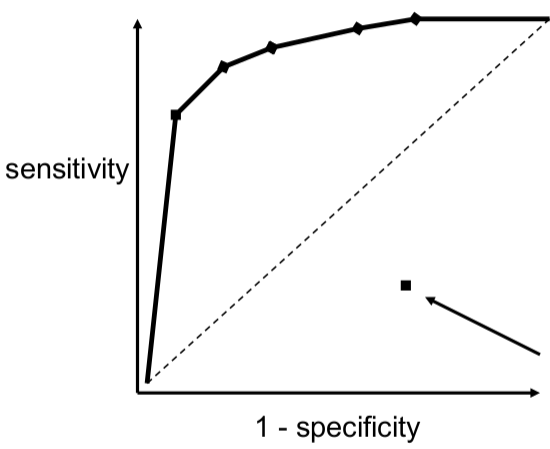
\includegraphics[width=0.4\textwidth]{roc_analysis}
		\caption{A sample ROC space}
		\label{fig:roc_analysis}
	\end{wrapfigure}
	
	All of the optimal detectors lie on the convex hull - the best possible position is for a detector to lie in the top left corner. It should be noted that if the edge detector lies below the dotted line then we can instantly make the detector better by simply just flipping the output of the algorithm!
		
	\section{Object Recognition}
	Object recognition\index{object recognition} aims to find objects in the real world from an image of the real world using previously known models. We could define this as a labelling problem based on models of known objects. In order to successfully recognise objects, we need the following components
	\begin{itemize}
		\item A model database, sometimes referred to as a model base
		\item A feature detector
		\item A hypothesizer
		\item A hypothesis verifier
	\end{itemize}

	The \textbf{model database} contains all models known to the system. Information in a model depends on the approach used for recognition. It may be precise geometric surface information or something more abstract such as a functional description. The \textbf{feature detector}\index{feature detector} applies operators to the image and identifies the location of features. This depends on the type of objects and organisation of the model database. The \textbf{hypothesizer}\index{hypothesizer} uses detected features in an image to assign likelihoods to the objects present. This reduces the search space by using certain features. The \textbf{hypothesis verifier}\index{hypothesis verifier} uses object models to verify the hypothesis to refine the likelihoods of objects.
	
	\par 
	This method is not without issues. We need to consider how exactly we should represent our models in the model base compared to how the object is in real life. For example a red ball may not always be circular if it is a bouncy ball. The representation should capture all relevant information and be well organised. Additionally, when extracting features we need to decide on the features to extract as we may only be interested in a select few kinds.
	
	\section{Model Based Object Recognition}
	In the 1970s David Marr defined a coherent approach to the study of vision. He stated that vision is primarily a complex information task with a goal of capturing and representing the various aspects of the world that are of use. For example, if we are looking for something right in front of us, we might not care about the information on the periphery as that's not in use. Marr saw the brain as being exactly the same as a very complex computer, and used his ideas to try and model the function of the visual system. His computational approach had three levels:
	\begin{itemize}
		\item \textbf{Computational theory}: What is the model trying to accomplish? What are the processes for?
		\item \textbf{Algorithmic level}: What algorithm is needed? What sort of process might be needed?
		\item \textbf{Mechanism level}: What mechanism is needed to implement the algorithm? For example, with the brain this would be its neurology.
	\end{itemize}
	
	The problem that presents itself is that we can't be entirely sure that these theories are truly representative of actual brain functions because we cannot infer an algorithm from the properties of cells. Marrs contribution was to the 'computational theory' step in the vision process.
	
	\par 
	According to Marr, vision was a process of reconstructing the 3D scene from 2D information. The vision system must therefore have representations of 3D geometric structures so selecting models and recovering their parameters from image data is a key task in vision. Marr's approach was based on three main representations: the primal sketch, the 2.5D sketch and the 3D model. The primal sketch is the description of the intensity changes in the image and their local geometry - intensity variations in the image are likely to correspond to the physical reality. The 2.5D sketch is the viewer centred description of orientation, contour and depth. The 3D model is the object centred representation of 3D objects.
	
	\par 
	The Model based approach takes a somewhat object-centred approach and states that object recognition involves finding axes of symmetry\index{axes of symmetry} to interpret objects. It also identifies the use of 'generalised cones'\index{generalised cones} in recognising things. For example, the brain may treat a human as a set of conical shapes, like a mannequin. This makes sense, as it would be very inefficient when looking at a person for the visual system to process every single hair on their head. Instead, Marr says we generalise it to get a general impression of 'hairiness'.
	
	\par 
	There is an infinite variety of objects - how would we go about storing, representing and accessing models of them efficiently? One possible solution is to use a small library of 3D parts, from which we will construct many complex models. There are many schemes which use this approach: generalised cylinders, Geons etc. Biederman's 'Recognition by Components Theory' proposes that visual input is matched against structural representations of objects in the brain, consisting of geons and their interrelations. One problem of this comes from the idea of model vs appearance. To demonstrate this - something may look very different if viewed from the side rather than straight on. As a result, we would have to build many many models to deal with the same object from different perspectives. An approach to fixing this was the use of statistics - for example using a SIFT based recognition. When recognising a model, if we have 75\% of the features with a 95\% match, we can be reasonably certain we have the correct model.
	
	\par 
	Another problem is proposed once we move to category level recognition. We no longer have exact correspondence between features. For example, two different cars may look roughly the same but not exactly and do not have the same features as one another such as the lights being in different places. We need to encode structure to fix this problem. We use various parts of the image separately in order to determine if and where an object of interest exists. We use smaller part detectors and make a judgement about whether an image has an object based on the relative positions in which the components exist.
	\newpage
	\listoffigures
	\printindex

\end{document}
